%!xelatex = 'xelatex --halt-on-error %O %S'

\documentclass{buaaemp}
\usepackage{braket}
\begin{document}

% 标题,作者
\emptitle{微波铁磁顺磁共振}
\empauthor{智朝晖}{崔益民}

% 奇数页页眉 % 请在这里写出第一作者以及论文题目
\fancyhead[CO]{{\footnotesize 智朝晖: 微波铁磁顺磁共振}}


%%%%%%%%%%%%%%%%%%%%%%%%%%%%%%%%%%%%%%%%%%%%%%%%%%%%%%%%%%%%%%%%
% 关键词 摘要 首页脚注
%%%%%%%%关键词
\Keyword{铁磁共振,谐振腔,共振线宽, 多晶, 朗德因子}
\twocolumn[
\begin{@twocolumnfalse}
\maketitle

%%%%%%%%摘要
\begin{empAbstract}
铁磁共振是指铁磁介质的电子自旋共振, 观察的对象是铁磁介质中的末成对电子。它利用磁性物质从微波磁场中吸收能量的现象, 与核磁共振、顺磁共振一样在磁学和固体物 磁化强度、居里点等重要参数。本实验利用扫场法,使用了DH1121型3cm固态信号发生器产生9GHz左右的微波辐射通入谐振腔,观察到了单晶的共振曲线,通过测量输出电流的大小和此时磁场来确定共振线宽和g因子。
\end{empAbstract}

%%%%%%%%首页角注,依次为实验时间、报告时间、学号、email
\empfirstfoot{2022-11-18}{2022-11-18}{20377365}{20377365@buaa.edu.cn}
\end{@twocolumnfalse}
]
%%%%%%%%!首页角注可能与正文重叠,请通过调整正文中第一页的\enlargethispage{-3.3cm}位置手动校准正文底部位置:
%%%%%%%%%%%%%%%%%%%%%%%%%%%%%%%%%%%%%%%%%%%%%%%%%%%%%%%%%%%%%%%%
%  正文由此开始
\wuhao 
%  分栏开始



\section{理论分析}
\label{theory}
由磁学理论可知, 物质的铁磁性主要来源于原子或离子在未满壳层中存在的末成对电子自旋磁矩。一块宏观的铁磁体包括许多磁畴, 在每一个磁畴中, 自旋磁矩平行排列产生自发磁化,但各个磁畴之间的取向并不完全一致,只有在外加磁场 $B$ 的作用下, 铁磁体内部的所有自旋磁矩才趋向同一方向, 并围绕着外磁场方向作进动, 这时的总磁矩或磁化强度可用  $\mathbf{M} $ 表示。

\subsection{经典理论}
从经典力学的角度,一个处在静磁场$\mathbf{B_0}$中的磁矩${\mu}$将会绕磁场匀速进动,频率为拉莫尔频率$\mathbf{\omega_0}=\gamma \mathbf{B_0}$。若在垂直于静磁场$\mathbf{B_0}$的平面内加一以$\mathbf{\omega_0}$转动的弱磁场,磁矩${\mu}$与静磁场$\mathbf{B_0}$的夹角会大幅度变化,此即共振现象。而由电子自旋磁矩导致的共振即为电子自旋共振。其进动方程和进动频率可经典地写为:

\begin{equation}
    \frac{d \mathbf{M}}{d t}=-\gamma(\mathbf{M} \times \mathbf{B}) \\
\omega=\gamma B
\end{equation}

\subsection{量子理论:磁矩与$g$因子}
	电子的轨道运动和自旋均会带来磁矩:
	$${\mu}=-\frac{g_0e}{2m_e}\mathbf{S}=\gamma \mathbf{S}$$
	
\newpage

 其中$g_0$为$g$因子,对于自由电子,$g_0\approx2.0023$。
	
从量子力学的角度,静磁场$\mathbf{B_0}$会使得电子的能级发生塞曼分裂,电子自旋向上和向下将会具有不同的能量,能级差为:$$\Delta E=g_0\mu_BB_0$$
	
	其中$\mu_B$为玻尔磁子。在静磁场和微波磁场的共同作用下,体系的哈密顿量为:$$H=-{\mu}\cdot\mathbf{B}=\gamma \mathbf{S}\cdot(\mathbf{B_0}+\mathbf{B_1}(t))$$
	
	若初始时电子的自旋为$\ket{+}$,根据拉比公式\cite{enwiki:1049655724},在$t$时刻测量到电子自旋为$\ket{-}$的概率为:$$P_{+-}(t)=\frac{\omega_{1}^{2}}{\omega_{1}^{2}+(\Delta \omega)^{2}} \sin ^{2}\left[\sqrt{\omega_{1}^{2}+(\Delta \omega)^{2}} \frac{t}{2}\right]$$
	
	其中$\omega_1=-\gamma B_1$,$\Delta \omega=\omega-\omega_0$,$\omega$为磁场$\mathbf{B_1}$的角频率\footnote{由于线偏振的磁场可以分解为两个圆偏振叠加,而这里面只有一个分量的角频率可以达到或接近共振频率(另一个是它的相反数),因此$\omega$也可以理解为外加旋转磁场的转动角速度。}。共振时$\Delta\omega=0$,$P_{+-}$在$[0,1]$之间取值,样品与磁场间有很强的能量交换,通过检测这一能量的变化即可观察电子自旋共振信号。

上述情况末考虑阻尼作用。在外加恒磁场  $B $ 作用下, 磁 矩 $ M  $绕  $B $ 进动不会很久, 因为铁磁物质的自旋磁矩与晶格或 邻近的磁矩存在着耦合作用, 即与周围环境之间存在着能 量的交换。由于铁磁介质内部有损耗存在, 使磁化强度矢 量 $ M $ 的进动受到阻力, 绕着外磁场 $ B $ 进动的幅角  $\theta$  会逐渐减 小。则 $ M$  最终趋近磁场方向, 这个过程就是磁化过程, 磁性 介质所以能被磁化, 就说明其内部有损耗, 如果要维持其 进动, 必页另外提供能量。因此一般来说外加磁场由两部 分组成: 一是外加恒磁场  $B$ , 二是交变磁场 $ H_{m}$  (即微波磁场) - 此时铁磁物质从微波磁场吸收的全部能量恰好补充铁磁 样品所损耗的能量。这正是铁磁共振可以用来研究铁磁材 料的宏观性能和微观机制之间关系的物理基础。
当外加微波磁场 $ H_{m}$  的角频率  $\omega_{0} $ 与礠化强度矢量$  M$  进动

磁学中通常用磁导率 $ \mu $ 来表示磁性材料被磁化的难易程度,在恒定磁场下 $\mu$可用实数表示: 在交变磁场下, $ \mu$  要用复数表示:

\begin{equation}
    \mu=\mu^{\prime}-i \mu^{\prime \prime}
\end{equation}

其中实部  $\mu^{\prime}$  为铁磁介质在恒定磁场中的磁导率,
它决定磁性材料中储存的磁能, 虚部  $\mu^{\prime \prime} $ 反映交变 磁场时磁性材料的磁能损耗。
当发生铁磁共振时, 铁磁体会出现一个最大 的磁能损耗, 磁导率的虚部  $\mu^{\prime \prime}$  与恒定磁场 $ \mathrm{B} $ 的 关系曲线上出现共振峰, 如图 所示。 $ \mu^{\prime \prime}$  的最大 值  $\mu_{r}^{\prime \prime} $ 对应的磁场  $B_{0}$  称为共振磁场。  $\frac{1}{2} \mu_{r}^{\prime \prime}$  两点对 应的磁场间隔 $ \left(B_{2}-B_{1}\right)$  称为铁磁共振线宽 $ \Delta \mathrm{B} $。 $\Delta \mathrm{B} $ 是铁磁材料的一个重要参量, 它的大小标志磁损耗的大小,一般 $\Delta B$越窄, 磁能损耗越低。
	
 \section{实验过程}
	\label{section:procedure}
	本实验利用DH1121B型三厘米固态信号源生成频率约为9000MHz的微波,微波经过隔离器、衰减器后进入波导到达样品处,再经隔离器后到达检波晶体处。样品置于电磁铁的两个水平圆形线圈之间,电磁铁由共振仪提供直流、交流励磁电流,磁场强度由SG-41型数字特斯拉计测量。共振仪的扫场信号和检波晶体的信号分别连接到GOS-6021型示波器的CH1和CH2通道。实验装置示意图见图\ref{figure:apparatus}:
	\begin{figure}[htbp]
		\centering
		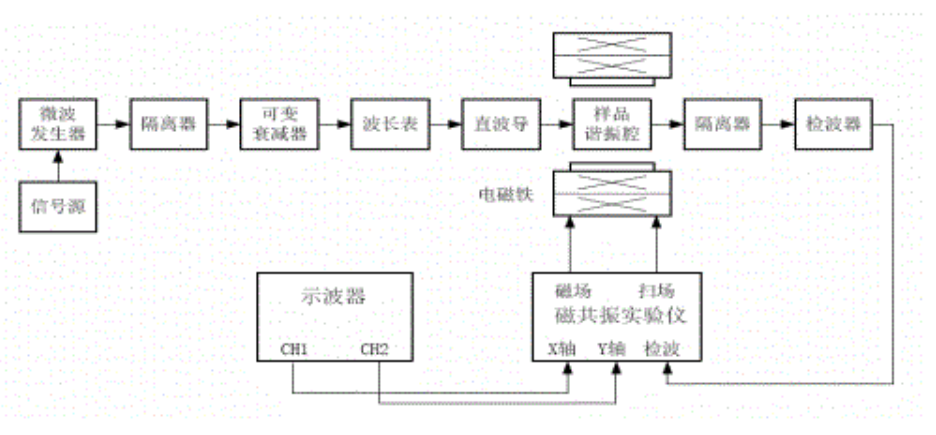
\includegraphics[width=\linewidth]{image/apparatus.png}
		\caption{实验装置示意图\cite{钱建强2016近代物理实验}}
		\label{figure:apparatus}
	\end{figure}
	
	实验开始前,打开固态信号源和特斯拉计预热半小时。实验正式开始后,首先调节谐振腔谐振,具体做法见下。按照实验室提供的“频率-测微器刻度对照表”,调节螺旋测微器示数。衰减器的衰减调为一个较大的值,波长计调为0,打开磁共振实验仪并调整为“检波”模式,转动“检波灵敏度”旋钮,使得表盘有一适中的示数,调节单螺调配器至表盘示数达到一极小值,随后增大“检波灵敏度”并减小衰减器的衰减,继续调节单螺调配器,直至表盘示数降为0(或接近0)。此时谐振腔达到谐振状态。
	
	调节单螺调配器的探针深度,使得“检波”有一较大的示数,转动波长计的旋钮,直至该示数降为0,记下此时波长计的读数,并对照实验室提供的“3cm空腔波长表频率刻度对照表(一)”得到谐振频率$f_0$。
	
	保持谐振频率不变,将波长计归零,调节单螺调配器的探针深度,使得“检波”示数为0.接下来观察单晶样品的共振曲线。将磁共振实验仪调整为“扫场”模式,示波器为“X-Y”显示,向右转动“磁场”旋钮,直至屏幕上出现共振信号;再将示波器调至“扫描”状态,即可观察到共振扫描信号。扫场电流置于最小,调节“磁场”使得各峰等间距排列,对得到的共振信号进行适当的放大、平移、相移,随后调节“磁场”旋钮直至两个共振峰变为一个,观察。
	
	最后测量共振线宽$\Delta H$,并计算朗德因子$g$。当微安表有理想示数后,加大磁场电流,测得 $I_0$ ,$I_r$, $H_r$ 。根据这些数据即可算得 $I_{\frac{1}{2}}=\frac{2I_0 I_r}{I_0 + I_r}$,读出此时对应的半功率点的磁场强度值 $H_1$ ,$H_2$, 得到$\Delta H=|H_1 -H_2|$,代入公式可得$g$。
	
	\section{数据记录及处理}
	\subsection{调节谐振腔至谐振频率}
	粗调3cm固态信号源的旋钮后,波长计读数为:$$x_{3cm}=3.578mm$$
	
	对应的频率为:$$f_{3cm}=8.935GHz$$
	\subsection{观察单晶共振信号}
	按照\ref{section:procedure}部分所述的步骤,可以观察到单晶共振信号,见图\ref{figure:one}:
	\begin{figure}[htbp]
		\centering
		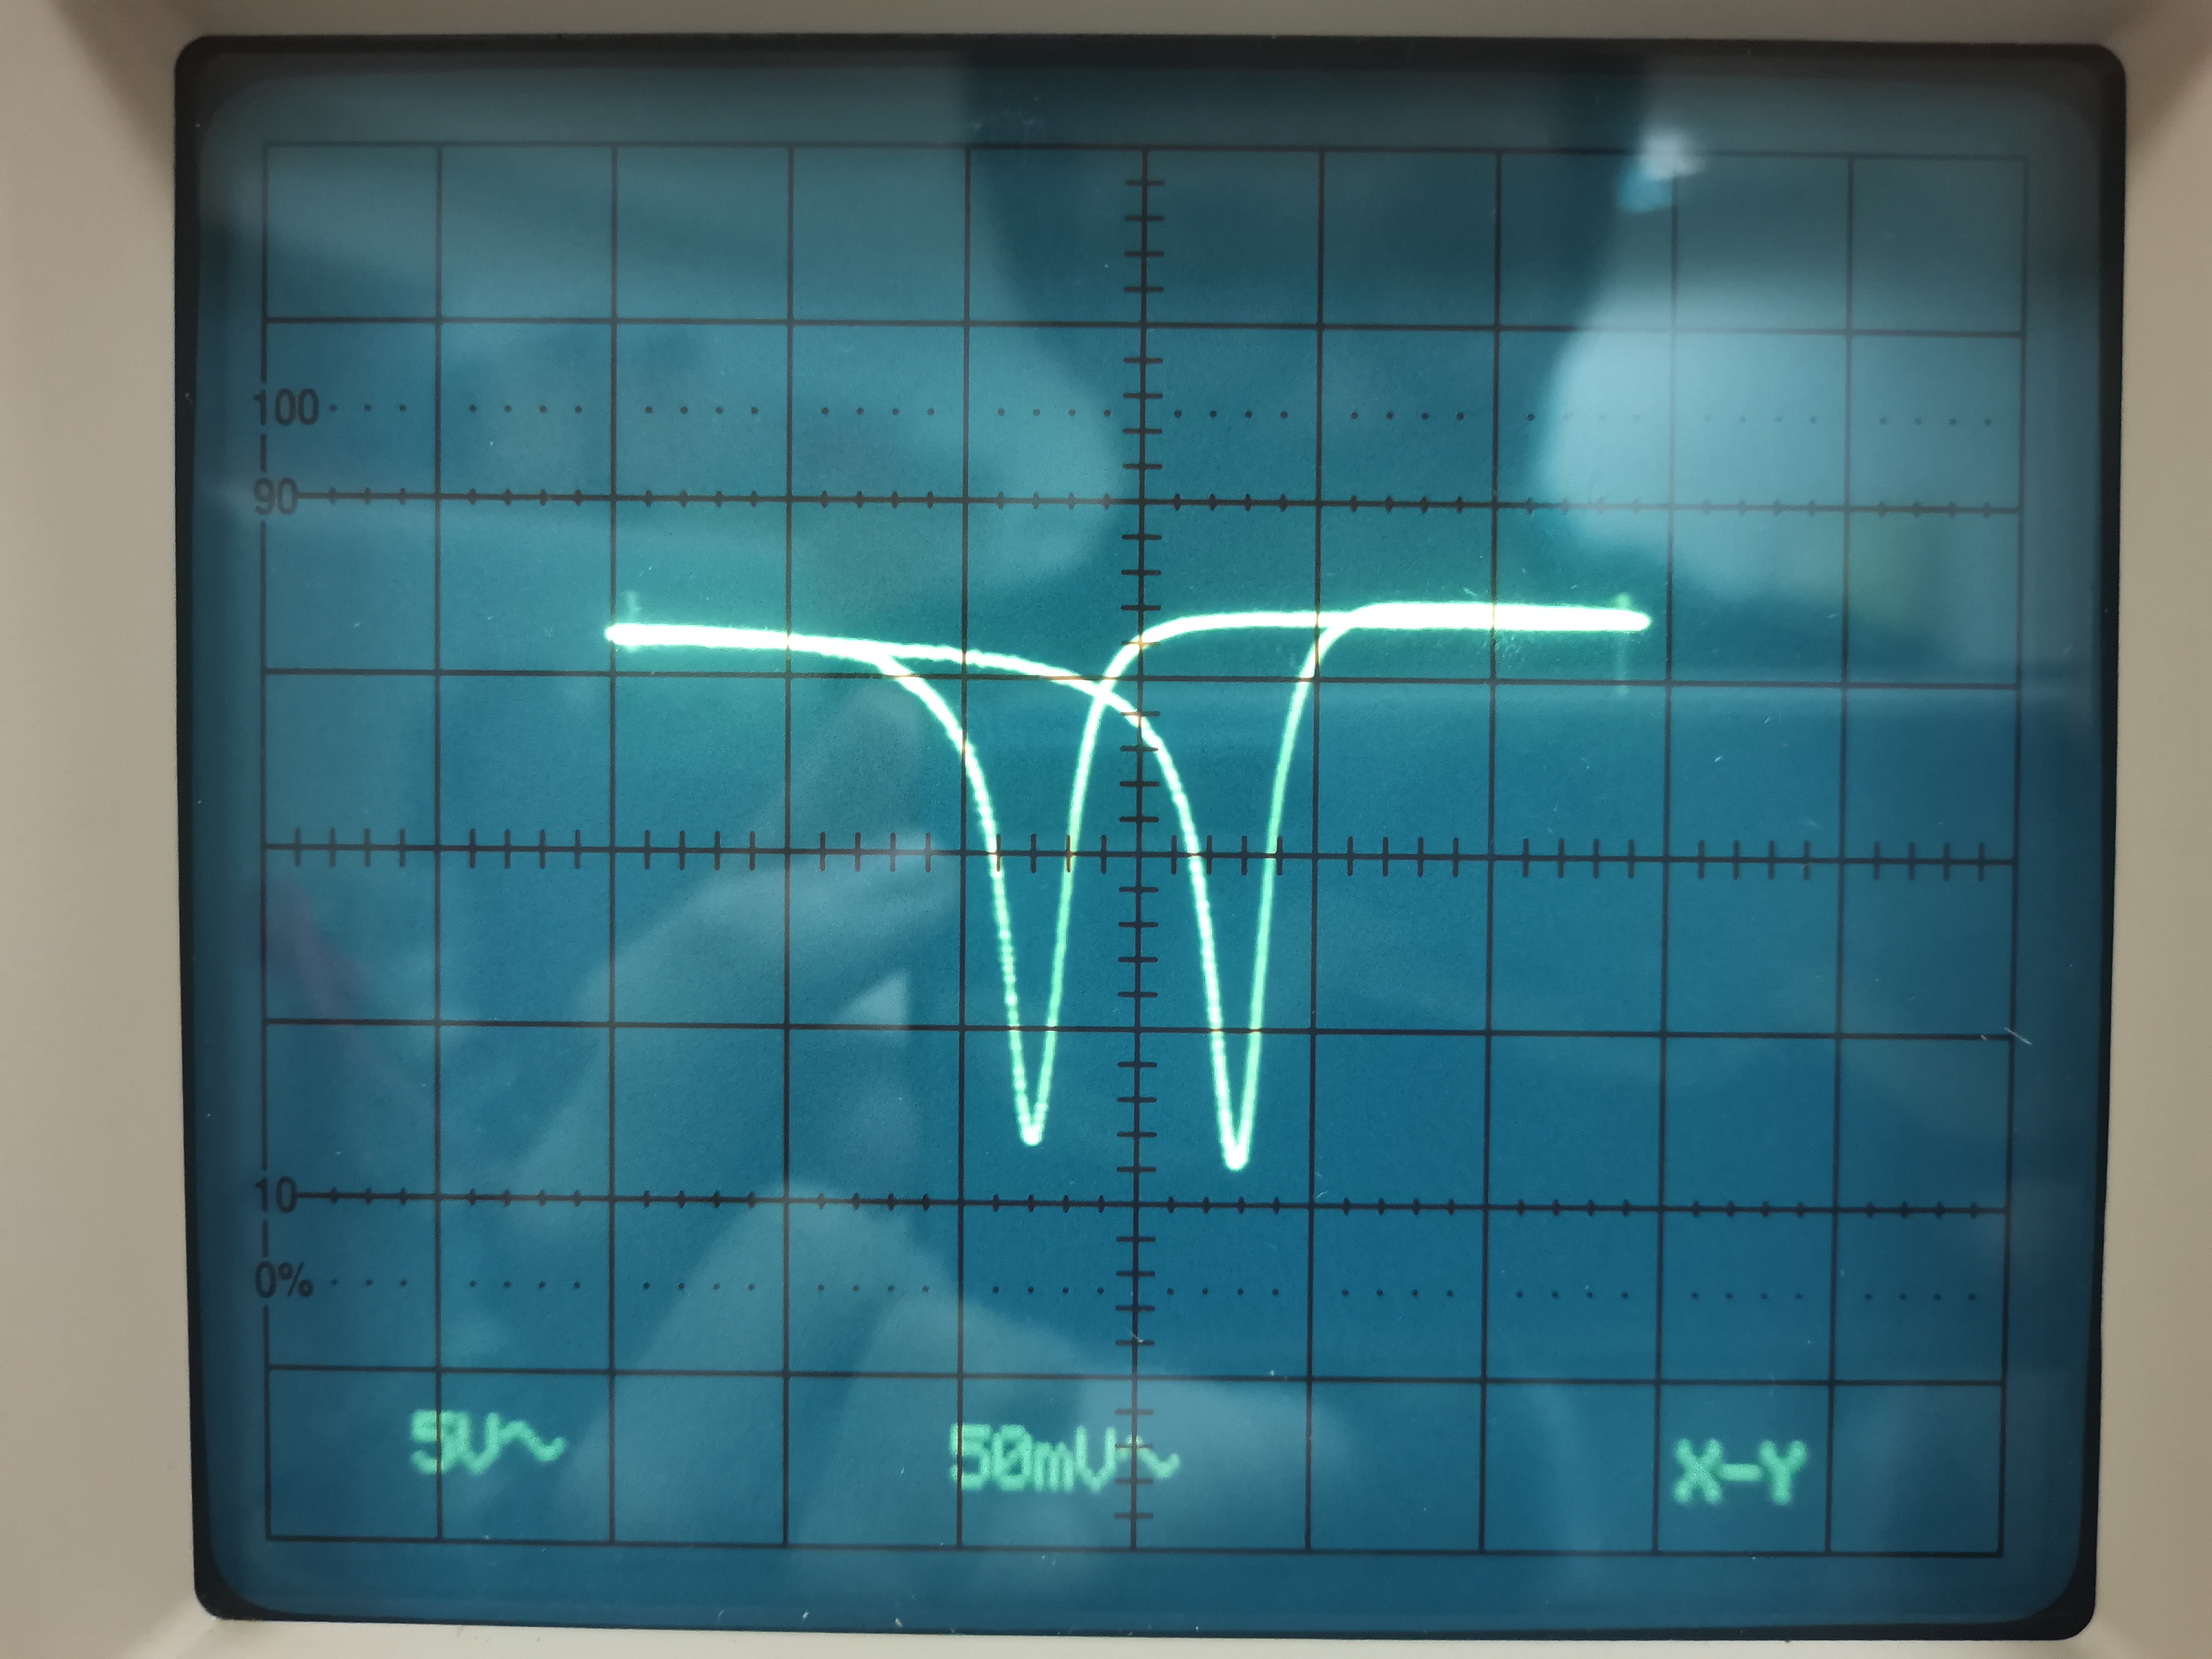
\includegraphics[width=\linewidth]{image/one.jpg}
		\caption{电子自旋共振信号}
		\label{figure:one}
	\end{figure}

	
	\begin{figure}[!htbp]
	
			\centering
			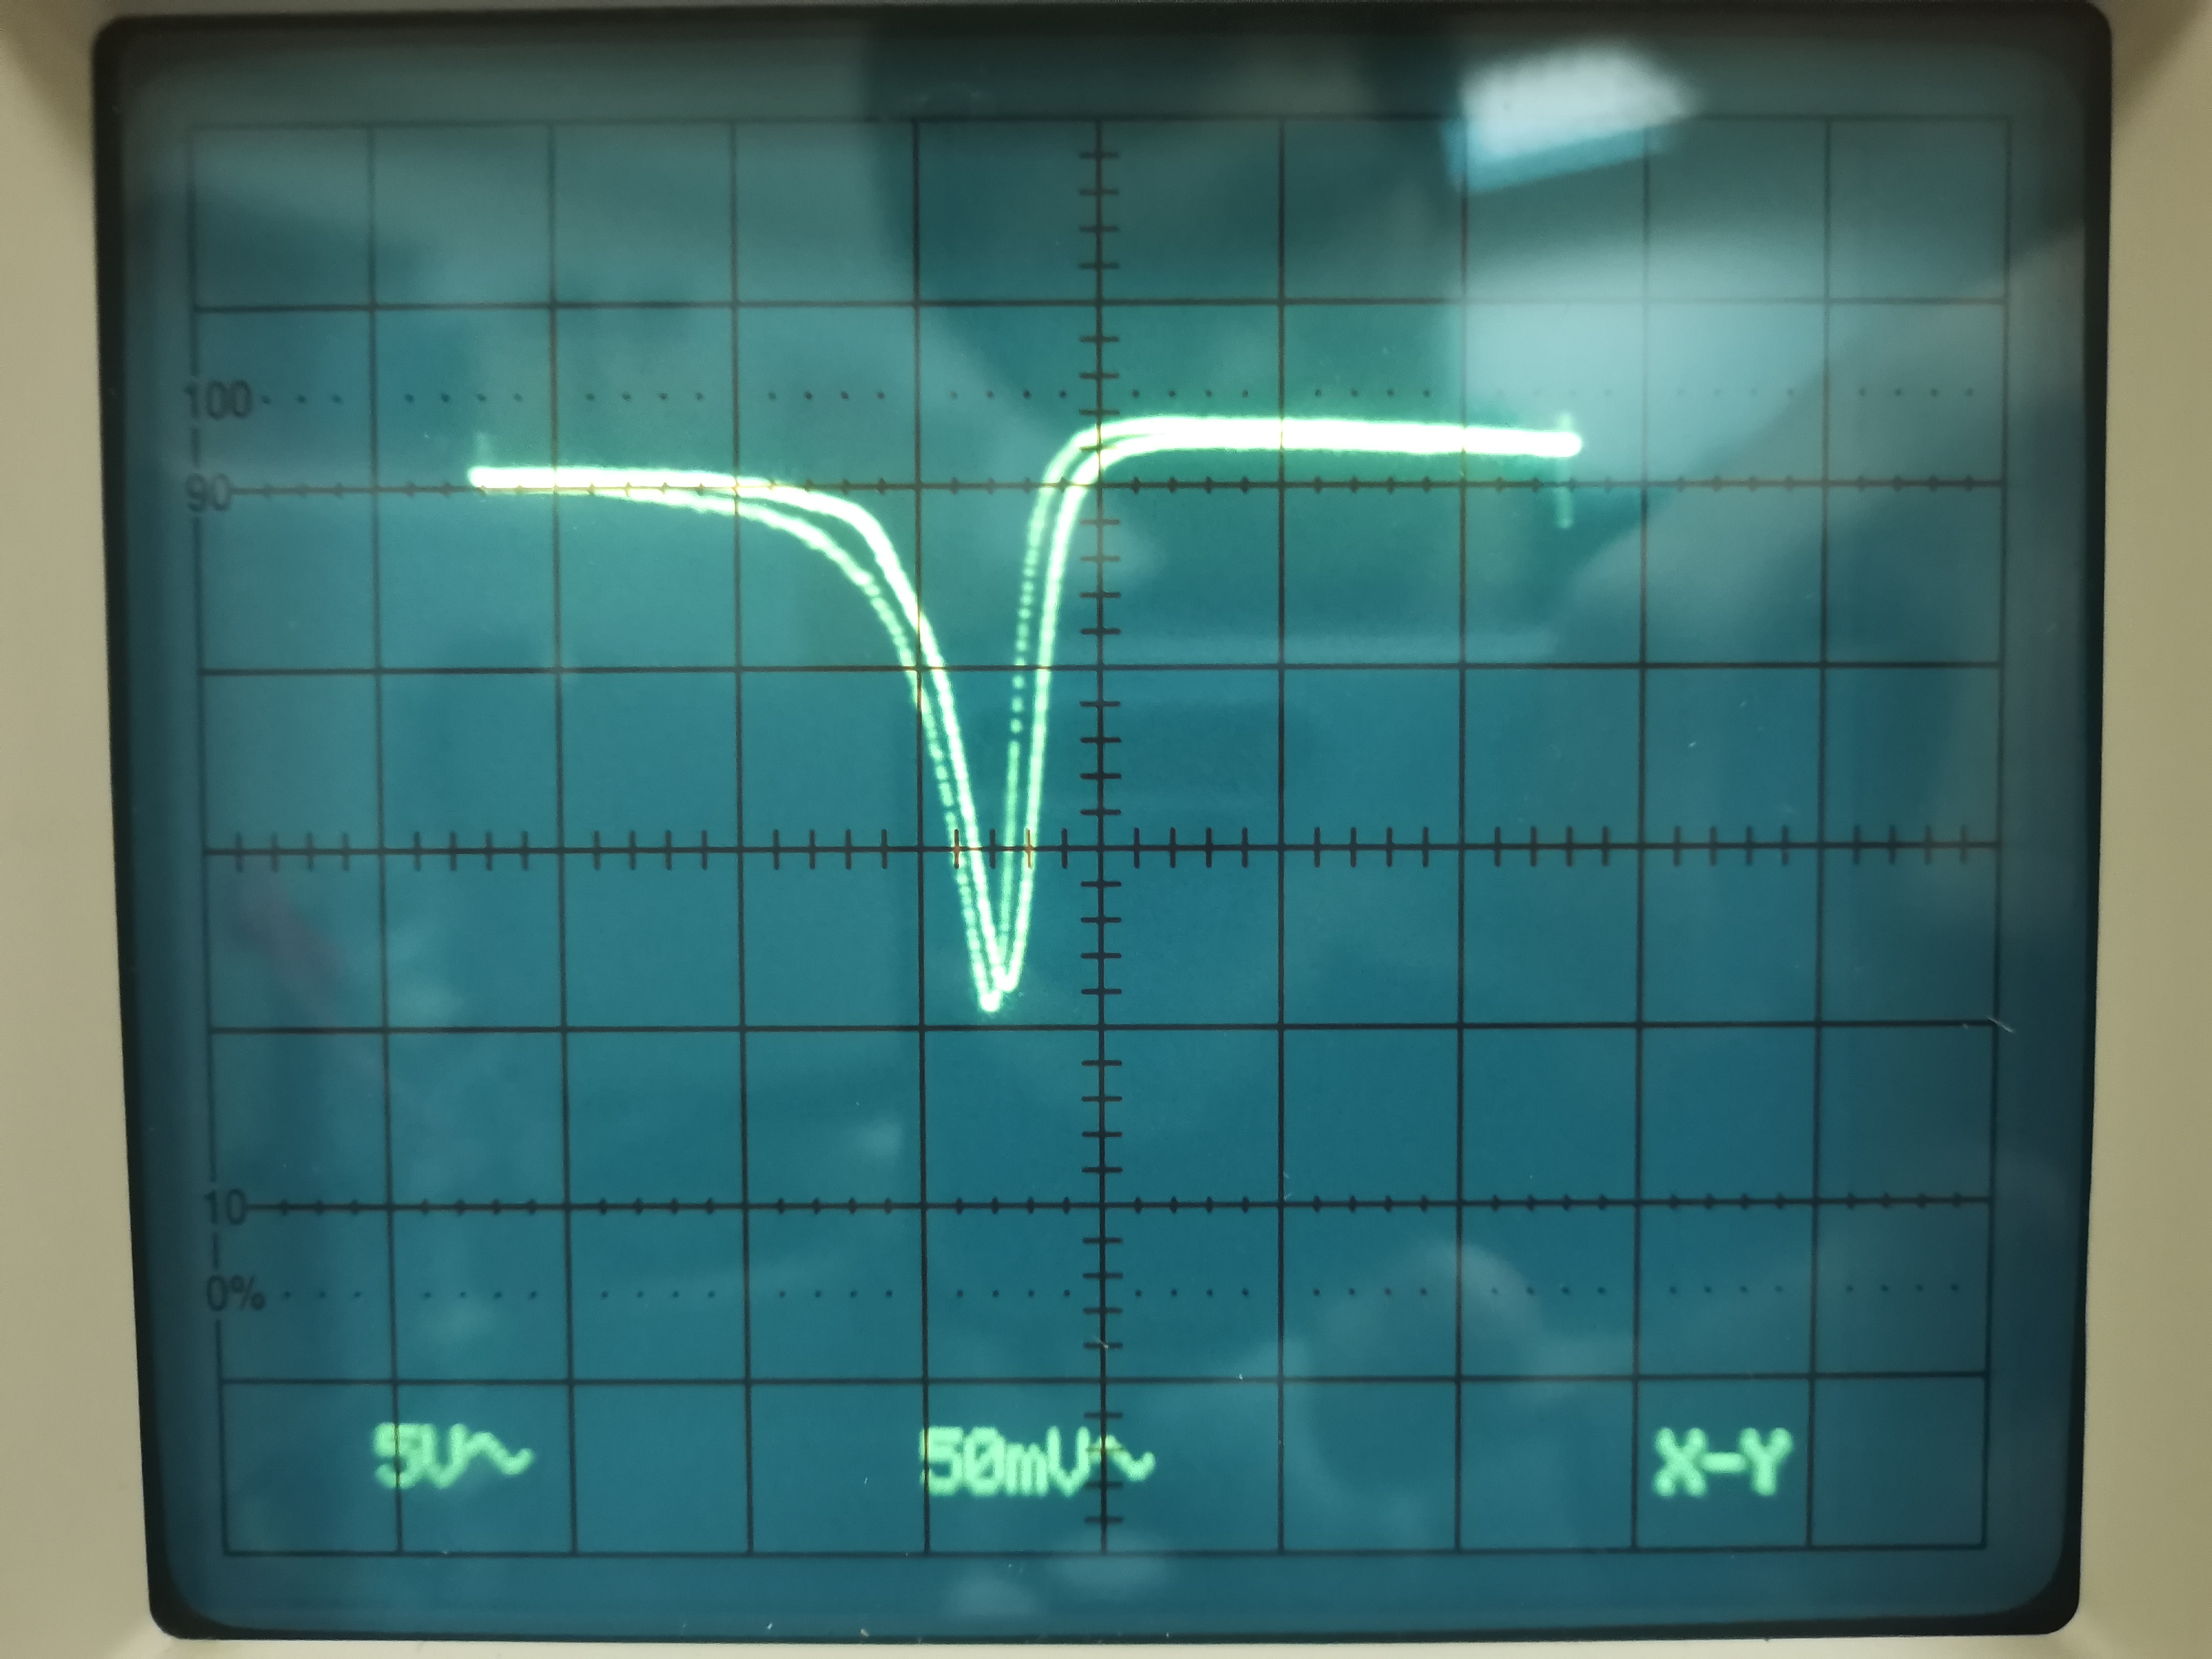
\includegraphics[width=\linewidth]{image/two.jpg}
   \end{figure}
		\begin{figure}
			\centering
			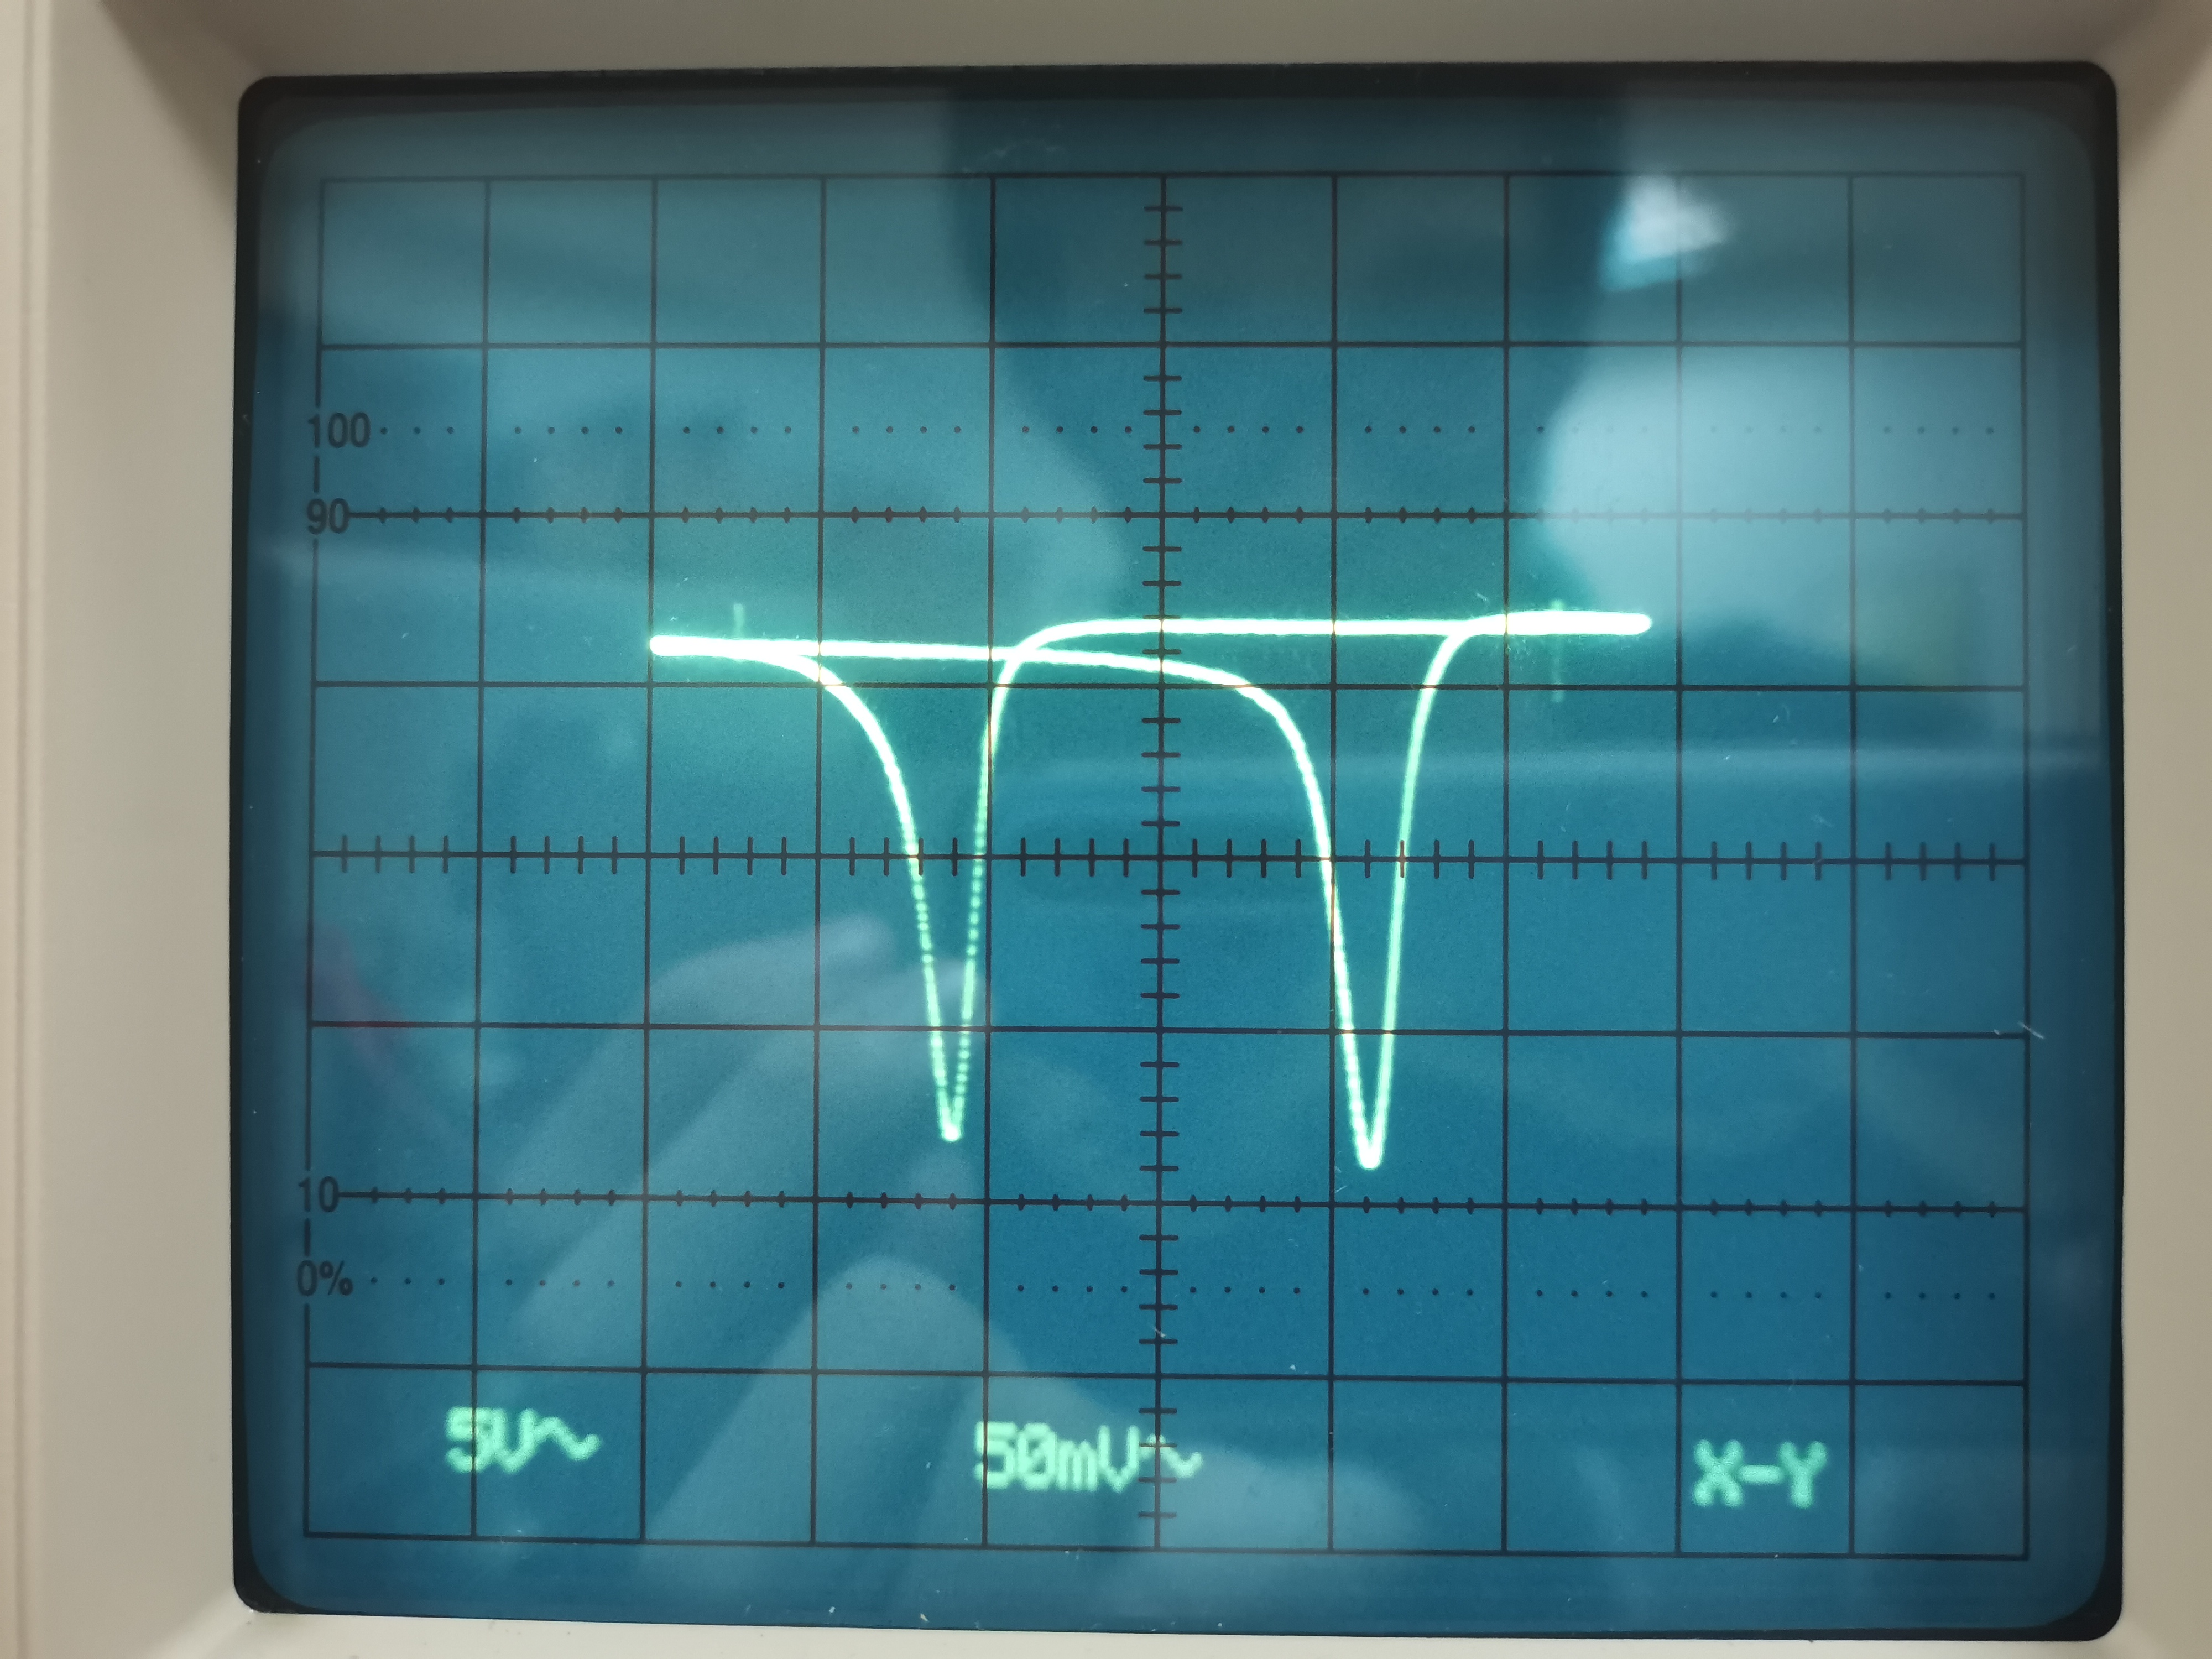
\includegraphics[width=\linewidth]{image/three.jpg}
		\caption{调节交流磁场相位使得两个共振峰发生移动}
		\label{figure:displacement}
	\end{figure}
 
\begin{figure}
        
            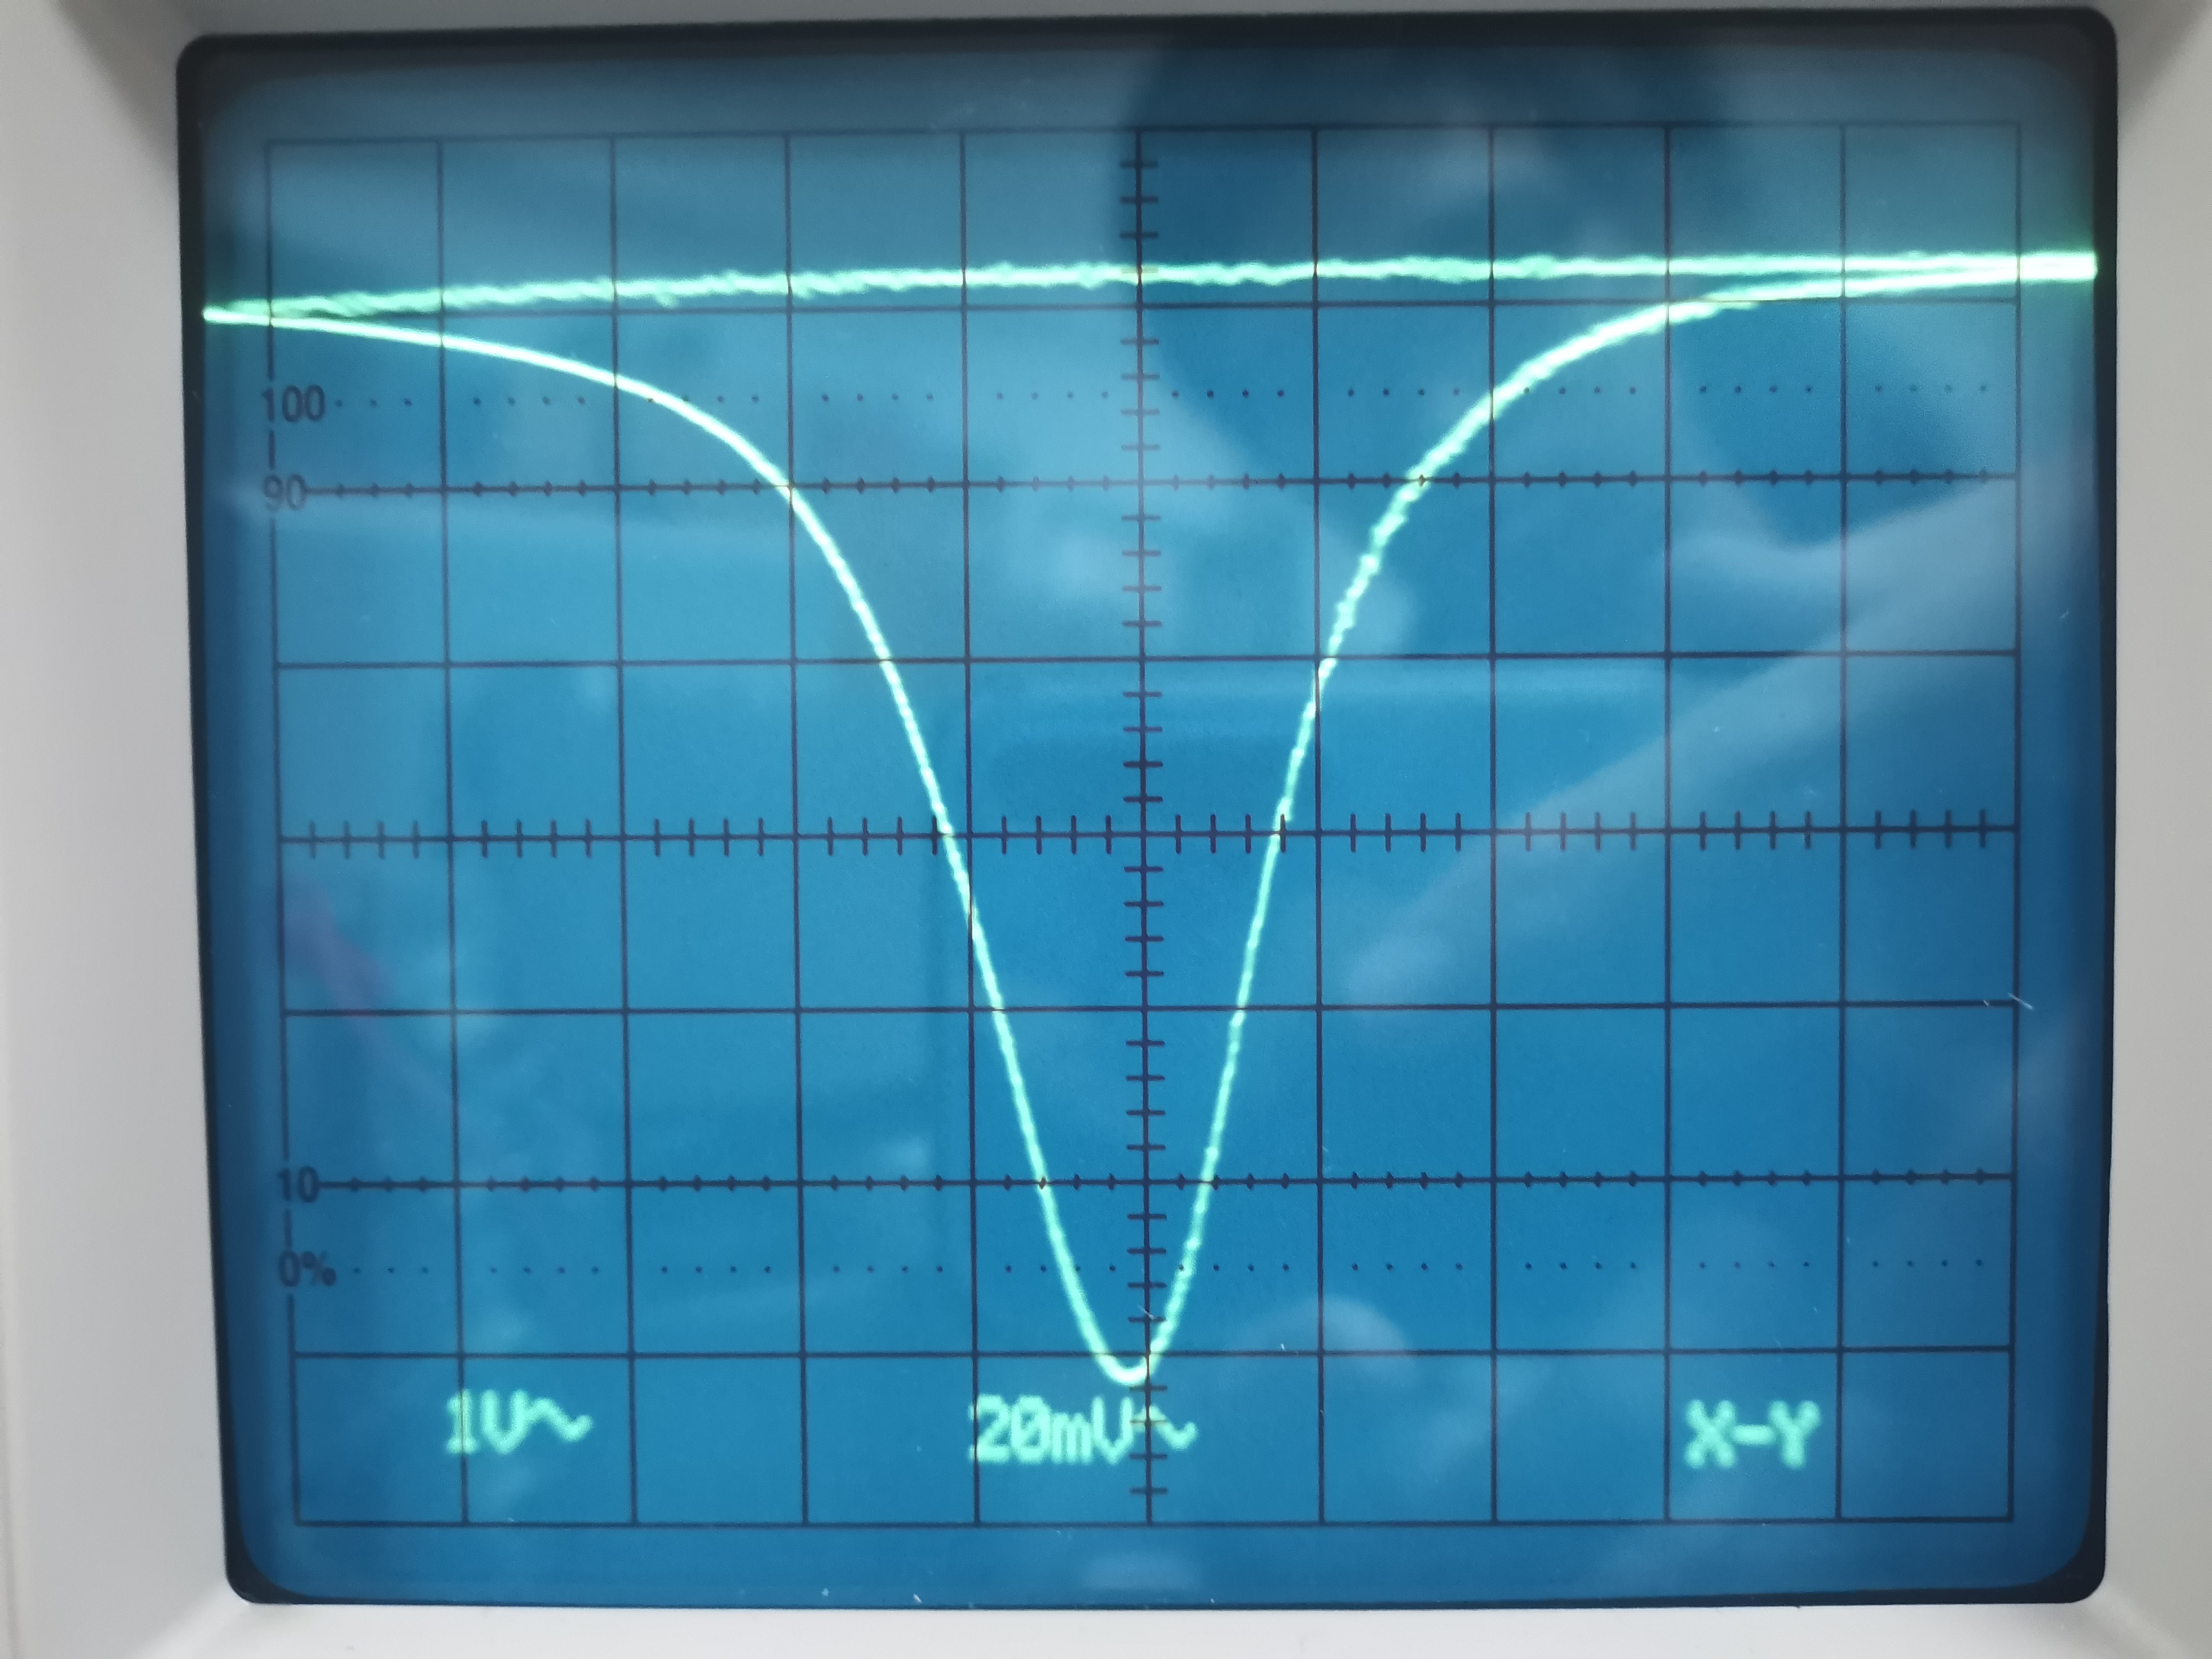
\includegraphics[width=\linewidth]{image/db2.jpg}
			\caption{调相后,两个峰在中间处变为一个峰}
			\label{figure:phase2}
		
	\end{figure}
	

	
	
\subsection{测量共振线宽和g因子}
 \ref{tabular:width}:
	\begin{center}
		\caption{共振线宽$\Delta H$的测量}
		\begin{tabular}{ccc}
			\hline\hline\noalign{\smallskip}
		磁场1/(T) & 磁场2/(T) & $\Delta H$/(T) \\
			\noalign{\smallskip}\hline\noalign{\smallskip}
			0.3104 & 0.3362 & 0.3233\\
            \hline\hline\noalign{\smallskip}
		$I_0 (\mu A)$ & $I_2(\mu A)$ & $I_{\frac{1}{2}} (\mu A)$ \\
		\noalign{\smallskip}\hline\noalign{\smallskip}
        124.5 &82.8 &99.4 \\
        \noalign{\smallskip}\hline\hline
		\end{tabular}
		\label{tabular:width}
	\end{center}
	
	计算可得共振线宽的值为:$$\bar{\Delta H}=25.8 mT$$,朗德因子 $g=\frac{2m \omega}{e \Delta H}$=1.98
	
	
	
	\section{总结}
	本实验利用“铁磁共振实验仪”,观察了单晶样品的共振曲线测量了多晶的$g$因子和共振线宽:
	$$g=1.98 $$
        $$\Delta H=25.8 mT$$
	
	\section{思考题}
	\begin{itemize}
	    \item 因为在信号强度较小时晶体检波器符合平方律,即检波电流与功率正比,故输出功率可用检波电流作相对指示,测得 $I-H$曲线就是 $P-H$曲线,而 $\mu^{\prime\prime} $ 也反映了能量损耗强度。即 $\mu^{\prime\prime} -H$曲线。 
            \item 如本文\ref{theory}部分
            \item 要保证此时微安表示数为 $I_{\frac{1}{2}}$,同时应该保证此时衰减和谐振腔腔长不变。
	\end{itemize}


%%%%%%%%%%%%%%%%%%%%%%%%%%%%%%%%%%%%%%%%%%%%%%%%%%%%%%%%%%%%%%%%
%  参考文献
%%%%%%%%%%%%%%%%%%%%%%%%%%%%%%%%%%%%%%%%%%%%%%%%%%%%%%%%%%%%%%%%
%  参考文献按GB/T 7714-2015《文后参考文献著录规则》的要求著录. 
%  参考文献在正文中的引用方法:\cite{bib文件条目的第一行}

\renewcommand\refname{\heiti\wuhao\centerline{参考文献}\global\def\refname{参考文献}}
\vskip 12pt

\let\OLDthebibliography\thebibliography
\renewcommand\thebibliography[1]{
  \OLDthebibliography{#1}
  \setlength{\parskip}{0pt}
  \setlength{\itemsep}{0pt plus 0.3ex}
}

{
\renewcommand{\baselinestretch}{0.9}
\liuhao
\bibliographystyle{gbt7714-numerical}
\bibliography{./TempExample}
}


\end{document}
